\chapter{FPGA usages in cryptography\label{FPGA_crypto}}
Due to the high demand on fast cryptographic methods, optimized implementations
became of huge interest. Hence the motivation behind developing faster FPGA
implementation of cryptographic schemes. In this chapter we are giving an
overview of optimized FPGA implementations for R-LWE.

\begin{figure}[H]

    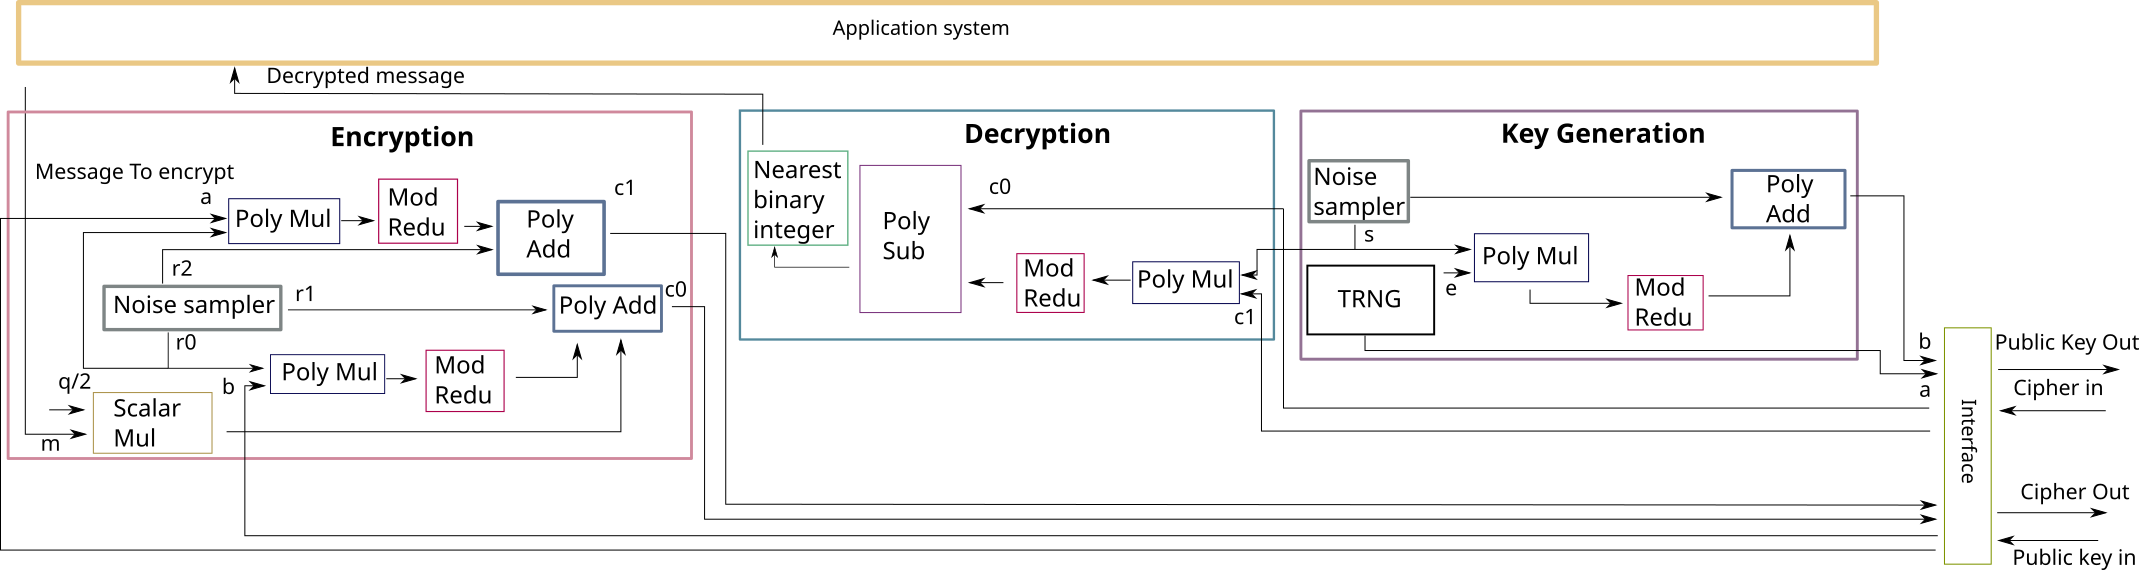
\includegraphics[scale=0.25]{high_level_impl.png}
    \caption{An optimized high level implementation of the three building
    blocks for a public key cryptosystem \citep{FPGA_Post_Quantum_Primitives}}
    \label{fig:high_level_pkc_impl}

\end{figure}

The implementation as seen in Figure \ref{fig:high_level_pkc_impl} consist of
three different modules: key generation, encryption and decryption. These
modules consist of a few basic operations, polynomial multiplication,
polynomial addition, subtraction and scalar division to the nearest integer.
The most expensive complexity-wise is the modulo operation which can take a few
hundred LUTs \citep{FPGA_Post_Quantum_Primitives}. Which is why these designs
try to minimize the amount of modulo operations with operations such as
conditional assignment.

\begin{itemize}
    \item
        Polynomial addition and subtraction is the most common operation in the
        R-LWE cryptosystem. It uses a hardware circuit to do the polynomial
        addition/subtraction and conditional assignment to avoid using the
        modulo operation.

    \item
        Scalar multiplication uses multiplexers to once again save LUTs as
        $m$ is an $n$-bit vector, when computing $t\cdot m$ we choose
        essentially$t$ or $0$.

    \item
        Scalar division to the nearest integer
    \item
        Polynomial multiplication

\end{itemize}
